\documentclass[journal]{IEEEtran}

\usepackage{amscd,amssymb}
\usepackage{amsfonts}
\usepackage{url}
\usepackage{xspace}
%\usepackage[pdfusetitle,colorlinks,plainpages=false]{hyperref}
%\usepackage{biblatex}
\usepackage{tikz}
\usepackage{tikz-qtree}
\usepackage{tikz-uml}
\usepackage[caption=false]{subfig}
\usepackage{tabularx}
\usepackage{color}
\usepackage{amsmath}
\usepackage{listings}
\usepackage{units}
%\usepackage{amsthm}
\usepackage{algpseudocode}
\usepackage{algorithm}
% \usepackage[T1]{fontenc} \usepackage{lmodern}

\newenvironment{keywords}{
       \list{}{\advance\topsep by0.35cm\relax\small
       \leftmargin=0cm
       \labelwidth=0cm
       \listparindent=0cm
       \itemindent
       \listparindent
       \rightmargin\leftmargin
       }
  \item[\hskip\labelsep
                                     \bfseries Keywords:]}
     {\endlist}

%\theoremstyle{definition}
\newtheorem{defn}{Definition}
\newtheorem{thm}{Theorem}
\newtheorem{corr}{Corollary}

\definecolor{dkgreen}{rgb}{0,0.6,0}
\definecolor{gray}{rgb}{0.5,0.5,0.5}
\definecolor{mauve}{rgb}{0.58,0,0.82}

\lstdefinelanguage{PIL}{
morekeywords={ExecutionOrder, Common, Prover, Verifier, Def, Void, Prime, Z, Int},
otherkeywords={Zmod+, Zmod*},
morecomment=[l]{//},
morecomment=[s]{/*}{*/}
}

\lstdefinelanguage{PSL}{
  morekeywords={Prime, Public, ProverPrivate,
    KnowledgeError, SZKParameter, ProtocolComposition, Homomorphism,
    ChallengeLength, SigmaPhi, Relation, Declarations, Inputs, Properties},
  otherkeywords={Zmod+, Zmod*},
  morecomment=[l]{//}, morecomment=[s]{/*}{*/}
}

\lstdefinelanguage{grammar}{
  keywords={},
  otherkeywords={}
}

\lstdefinelanguage{GEZEL}{
  morekeywords={sfg, dp, always, reg, syg, system, ns, tc, out, in, use, sig},
  otherkeywords={$display, $hex, $dec, $bin, $cycle},
  morecomment=[l]{//}
}

\lstset{
language=PIL,
basicstyle=\footnotesize,
commentstyle=\color{dkgreen},
keywordstyle=\bfseries,
frame=single,
breaklines=true,
breakatwhitespace=false
}

\usetikzlibrary{backgrounds,calc,shapes,shapes.geometric,shadows,arrows,chains,trees,fit,positioning}

\tikzstyle{language}=[rectangle,draw=black,thin,inner sep=3pt, align=center]

\tikzstyle{compiler}=[rectangle,rounded corners,draw=black,thin,inner
sep=3pt, align=center]

\tikzstyle{added}=[fill=gray]

\begin{document}

\title{Implementation and Evaluation of Zero-Knowledge Proofs of Knowledge}

\author{
Boran Car, Josep Balasch, Alfredo Rial, Ingrid Verbauwhede and Bart Preneel}

\maketitle

\begin{abstract}
  Zero-knowledge proofs of knowledge (ZKPK) are the key building block
  of numerous cryptographic schemes, such as anonymous authentication
  or anonymous e-cash. Implementing ZKPK has proved to be error-prone,
  which hinders the widespread deployment of such schemes. To ease
  implementation work, several cryptographically aware compilers and
  libraries have been proposed to provide ZKPK implementations in
  high-level languages such as C, C++ and Java. However, some
  cryptographic schemes are expected to be implemented in
  resource-constrained devices, such as RFID tags (anonymous
  authentication) or smart cards (anonymous e-cash). In such
  situations, a ZKPK compiler that targets hardware description
  languages and hardware-software co-design is convenient.

  We propose a custom ZKPK compiler framework that extends the CACE
  ZKPK compiler to enable hardware-software co-design. Concretely, our
  ZKPK compiler takes as input platform-independent implementations
  generated by the CACE ZKPK compiler and transforms them into
  implementations in LLVM IR, the representation language of the LLVM
  compiler framework. From LLVM IR, one can target multiple
  platforms. We provide a back-end for GEZEL, a hardware description
  language which also enables hardware-software co-design. We also
  provide a back-end for C+GMP, thus covering both ends of the
  co-design spectrum. To demonstrate the flexibility of our framework,
  we take an existing system and implement Schnorr's Identification
  Protocol atop it in an automated way.

\end{abstract}

\begin{IEEEkeywords}
  zero-knowledge proof of knowledge, cryptographically aware
  compilers, hardware-software co-design
\end{IEEEkeywords}

%%% Local Variables:
%%% TeX-PDF-mode: t
%%% TeX-master: "paper"
%%% End:


\section{Introduction}
\label{introduction}
\chapter{Introduction}

\section{Zero Knowledge Proofs of Knowledge}

Today's state-of-the-art cryptosystems are based on the following hard
problems:
\begin{itemize}
\item Discrete Logarithm Problem
\item Factorization Problem
\end{itemize}

Such problems are not solvable using deterministic Turing machines
within polynomial time.  As long as computers are based on
deterministic Turing machines this does not pose as problem.  Simply
scaling the solution space has provided an effective countermeasure so
far. This is all about to change as the world sees the emergence of
quantum computers.

In a post-quantum computer world we would like to seek other problems
which are again not solvable within polynomial time using the machines
of the present.

Another motivation is that in our modern world, privacy is of the
uttermost importance. Let's look at a couple of everyday examples:
\begin{itemize}
\item Buying a public-transport ticket
\item Voting
\item Filling out anonymous questionnaires
\end{itemize}

So far, using traditional methods, privacy was not a big issue here. For
each of the cases:
\begin{itemize}
\item you paid for a piece of paper that nobody (unless he hires
  forensic) could connect to you
\item you circled your vote and put it in a box that nobody (again,
  unless he uses sophisticated methods) could connect to you
\item you filled in your questionnaire that nobody could connect to
  you
\end{itemize}

The real problem comes from trying to put these things into electronic
form. Using smart cards for public transport poses a big problem
w.r.t. privacy as nothing assures the user that the system does not
track him/her. The advantage of putting these things into electronic
form is multiple:
\begin{itemize}
\item less paper is wasted (smaller footprint)
\item less clutter if multiple smart cards are merged into a single
  one
\item less chance of the user losing his smart card if he only has one
\end{itemize}

However, one disadvantage strikes more than the others. The
possibility of the system to track the user and the user being
incapable of protecting his privacy. Traditional authentication
schemes required the user identifying himself so this tracking step
was an inherent property.

The desired property here is not disseminating any knowledge while
still proving to the system that certain properties hold (e.g. the
user has privileges and is allowed to proceed with an action).

\section{HW-SW codesign}

Traditional embedded device programming was separate from hardware
design. The separation went to such extents as having two separate
entities within a company working on each of those fields. The
software part is generic while the hardware part is faster and more
energy efficient.

Today's stringent measures require a bigger inter-dependency. Instead
of searching for a best algorithm tailored for specific hardware or
searching for the best hardware tailored to a specific algorithm/task,
why not design the hardware and software at the same time. This way
bigger decision and trade-offs can be made more granular
\cite{softeninghw}.

\begin{figure}[hbt!]
  \centering
  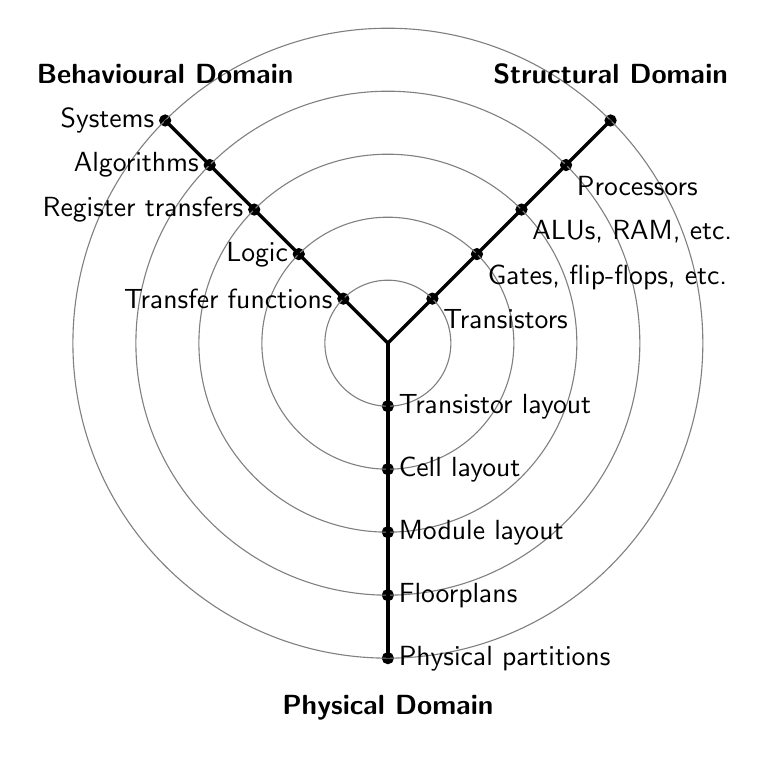
\begin{tikzpicture}[>=stealth',font=\sffamily,auto,on grid]
    %\input{y_chart_common}
    \coordinate (behaviouralNode) at (135:4cm);
    \coordinate (structuralNode) at (45:4cm);
    \coordinate (physicalNode) at (270:4cm);
    \coordinate (originNode) at (0:0cm);

    \draw[fill] (barycentric cs:behaviouralNode=1.0,originNode=0) circle (2pt);
    \draw[fill] (barycentric cs:behaviouralNode=0.8,originNode=0.2) circle (2pt);
    \draw[fill] (barycentric cs:behaviouralNode=0.6,originNode=0.4) circle (2pt);
    \draw[fill] (barycentric cs:behaviouralNode=0.4,originNode=0.6) circle (2pt);
    \draw[fill] (barycentric cs:behaviouralNode=0.2,originNode=0.8) circle (2pt);

    \draw[fill] (barycentric cs:structuralNode=1.0,originNode=0) circle (2pt);
    \draw[fill] (barycentric cs:structuralNode=0.8,originNode=0.2) circle (2pt);
    \draw[fill] (barycentric cs:structuralNode=0.6,originNode=0.4) circle (2pt);
    \draw[fill] (barycentric cs:structuralNode=0.4,originNode=0.6) circle (2pt);
    \draw[fill] (barycentric cs:structuralNode=0.2,originNode=0.8) circle (2pt);

    \draw[fill] (barycentric cs:physicalNode=1.0,originNode=0) circle (2pt);
    \draw[fill] (barycentric cs:physicalNode=0.8,originNode=0.2) circle (2pt);
    \draw[fill] (barycentric cs:physicalNode=0.6,originNode=0.4) circle (2pt);
    \draw[fill] (barycentric cs:physicalNode=0.4,originNode=0.6) circle (2pt);
    \draw[fill] (barycentric cs:physicalNode=0.2,originNode=0.8) circle (2pt);

    \draw[black!50] (0,0) circle (4.0cm);
    \draw[black!50] (0,0) circle (3.2cm);
    \draw[black!50] (0,0) circle (2.4cm);
    \draw[black!50] (0,0) circle (1.6cm);
    \draw[black!50] (0,0) circle (0.8cm);

    \node [above=1em] at (behaviouralNode) {\textbf{Behavioural Domain}};
    \node [above=1em] at (structuralNode) {\textbf{Structural Domain}};
    \node [below=1em] at (physicalNode) {\textbf{Physical Domain}};

    \draw[-, very thick] (behaviouralNode.south) -- (0,0) node[left,pos=0]{Systems} node[left,pos=0.2]{Algorithms} node[left,pos=0.4]{Register transfers} node[left,pos=0.6]{Logic} node[left,pos=0.8]{Transfer functions};

    \draw[-, very thick] (structuralNode.south) -- (0,0) node[pos=0]{ } node[pos=0.2]{Processors} node[pos=0.4]{ALUs, RAM, etc.} node[pos=0.6]{Gates, flip-flops, etc.} node[pos=0.8]{Transistors};

    \draw[-, very thick] (physicalNode.south) -- (0,0) node[right,pos=0]{Physical partitions} node[right,pos=0.2]{Floorplans} node[right,pos=0.4]{Module layout} node[right,pos=0.6]{Cell layout} node[right,pos=0.8]{Transistor layout};

  \end{tikzpicture}
  \caption{Gajski-Kuhn \index{Gajski-Kuhn Y-chart}Y-chart} 
  \label{figure:gajski_kuhn_y_chart__levels_of_abstraction}
\end{figure}

\filbreak

\section{Domain specific languages}

C and C++ are currently the dominant languages for embedded system
programming. It is therefore natural to expect that real-world
embedded cryptography applications be implemented in either of those
two languages. This can lead to hidden and difficult problems to
debug. A lot of cases were left unspecified or undefined in the C or
C++ standard. Hence, compiler implementations have a choice on how to
implement it. The usual approach is to define it as what is most
efficient in terms of the platform. This sacrifices the safety and
portability to ensure efficiency.

\filbreak

\begin{lstlisting}[language=C]
#include <stdio.h>

int b(void) { puts("3"); return 3; }
int c(void) { puts("4"); return 4; }

int main(void)
{
  int a = b() + c();
  printf("%d\n", a);
}
\end{lstlisting}

The evaluation order is unspecified so depending on the compiler, the
output may be 3, 4, 7 or 4, 3, 7. The compiler usually chooses the
optimal way to calculate it given a platform.

The security world does not handle undefined and unspecified values
well. It makes sense to build protections against unsafe, undefined
and unspecified operations into the language. It also makes sense to
make the language easy to learn and understand. This is the common
requirement of a domain specific language, a language tailored for a
specific domain.

%%% Local Variables: 
%%% TeX-PDF-mode: t
%%% TeX-master: "thesis"
%%% End: 


\section{Related Work}
\label{relatedwork}

The need for cryptographically aware compilers is extensively motivated by Bangerter et al.~\cite{citeulike:7079130}. A number of compiler based tools have been proposed recently. Some target a wide variety of cryptographic primitives and protocols~\cite{DBLP:conf/weworc/LucksST05,DBLP:conf/issa/BangerterKSU11}, while others focus on specific areas, such as multiparty computation~\cite{DBLP:conf/uss/MalkhiNPS04,DBLP:conf/pkc/DamgardGKN09,DBLP:conf/ccs/HeneckaKSSW10} and ZKPK.

A first example of ZKPK compiler was proposed in~\cite{TUD-CS-2005-0034} and extended in \cite{DBLP:conf/europki/BangerterBHKSS09}. Subsequently, Almeida et al. proposed the CACE ZKPK compiler~\cite{CACE}, which allows the implementation of most relevant $\Sigma$-protocols. The CACE ZKPK compiler avoids security vulnerabilities by choosing certain security parameters automatically and by validating the implementations via a formal theorem prover. A more detailed description is given in Section~\ref{sec:tools}.

Another ZKPK compiler (ZKPDL) was proposed by Meiklejohn et al.~\cite{Meiklejohn:2010:ZLS:1929820.1929838}. When compared to CACE, ZKPDL improves efficiency by using precomputation, but allows the implementation of a narrower class of protocols and does not provide formal verification. A detailed comparison between CACE and ZKPDL is given in \cite{Bangerter_yaczk:yet}.

To the best of our knowledge, currently there is no compiler that targets HW specification languages or that allows for HW-SW co-design.

 



%-	ZKPDL
%-	Other related work (take from the paper “A Certifying Compiler for Zero-Knowledge Proofs of Knowledge Based on Sigma-Protocols”

%%% Local Variables:
%%% TeX-PDF-mode: t
%%% TeX-master: "main"
%%% End:


\section{Background}
In this section we review necessary background information. In the
first part, we describe the targeted ZKPK $\Sigma$-protocols and in
the second part, we provide definitions of data flow graph and
control flow graph.
\label{preliminaries}
\chapter{Technical preliminaries}

The chapter has the goal of introducing the math and theory behind
formal languages, parsers, algebra, (zero knowledge) proofs of
knowledge.

\section{Formal Languages \cite{Hopcroft}}

\begin{defn}[Alphabet]
  An alphabet $\Sigma$ is a set of symbols.
\end{defn}

\begin{defn}[String]
  A string over an alphabet $\Sigma$ is a sequence of symbols of $\Sigma$.
\end{defn}

\begin{defn}[Concatenation]
  Let $x = a_0 a_1 \dotsm a_n$ and $y = b_0 b_1 \dotsm b_n$, then the
  string $x y = a_0 a_1 \dotsm a_n b_0 b_1 \dotsm b_n$ is the
  concatenation of the strings $x$ and $y$.
\end{defn}

\begin{defn}[Sets]
  The $\Sigma^*$ denotes the set of all the strings over the alphabet
  $\Sigma$, likewise $\Sigma^+$ denotes the set of all the non-empty
  strings over the alphabet $\Sigma$. $$\Sigma^+ \subseteq \Sigma^*
  \setminus \{ \epsilon \}$$ The empty set of strings is denoted
  $\emptyset$.
\end{defn}

\begin{defn}[Language]
  A language over the alphabet $\Sigma$ is a set of strings over
  $\Sigma$. Members of the language are called words of the language.
\end{defn}

\begin{defn}[Concatenation]
  Let $L_1$ and $L_2$ be two languages over alphabet $\Sigma$, the
  language $L_1 L_2 = \{x y | x \in L_1, y \in L_2 \}$ is the
  concatenation of $L_1$ and $L_2$.
\end{defn}

\begin{defn}[Kleene closure]
  Let $L$ be a language over $\Sigma$. Define 
  $$L^0 = \{ \epsilon \}$$
  $$L^i = L L^{i-1} \textrm{for} i \ge 1$$
  the \emph{Kleene closure} of $L$, denoted by $L^*$ is the language:
  $$ L^* = \bigcup_{i \ge 0} L^i $$
  the \emph{positive closure} is
  $$ L^+ = \bigcup_{i \ge 1} L^i $$
  It can be observed that
  $$ L^* = L^+ \cup \{ \epsilon \} $$
  $$ L^+ = L L^* $$
\end{defn}

\subsection{Regular expression}

\begin{defn}[Regular expression]
  A regular expression over $\Sigma$ is defined inductively as follows:
  \begin{enumerate}
  \item $\emptyset$ is a regular expression and represents the empty language
  \item $\epsilon$ is a regular expression and represents the language
    $L = \{ \epsilon \}$
  \item For each $c \in \Sigma$, $c$ is a regular expression and
    represents the language $L = \{ c \}$
  \item For any regular expressions $r$ of language $R$ and $s$ of language $S$:
    \begin{itemize}
    \item $r+s$ is a regular expression representing language $R \cup S$
    \item $r s$ is a regular expression representing language $R S$
    \item $r^*$ is a regular expression representing language $R^*$
    \item $r^+$ is a regular expression representing language $R^+$
    \end{itemize}
  \end{enumerate}
\end{defn}

\begin{thm}
  $r r^*$ can be represented as $r+$
\end{thm}

\begin{proof}
  $r r^*$ represents the language $R R^*$ which is $R^+$
\end{proof}

\subsection{Grammars}

\begin{defn}[Grammar]
  A grammar is a 4-tuple $G = \left< \Sigma, V, S, P \right>$:
  \begin{enumerate}
  \item $\Sigma$ is a finite non-empty set called the \emph{terminal
    alphabet}. The elements of $\Sigma$ are called \emph{terminals}.
  \item $V$ is a finite non-empty set disjoint from $\Sigma$. The
    elements of $V$ are called \emph{non-terminals} or \emph{variables}.
  \item $S \in V$ is a distinguished symbol called the \emph{start symbol}
  \item $P$ is a finite set of \emph{productions (rules)} of the form
    $$ \alpha \rightarrow \beta $$
    $$ \alpha \in (\Sigma \cup V)^* V (\Sigma \cup V)^* $$
    $$ \beta \in (\Sigma \cup V)^* $$
  \end{enumerate}
\end{defn}

\begin{defn}[Context-free grammar]
  The grammar $G$ is a context free grammar if $|\alpha|$ = 1 ($\alpha = V$).
\end{defn}

\begin{defn}[LL grammar]
  A context free grammar $G$ is an LL grammar if $\beta \in \Sigma
  (\Sigma \cup V)^*$
\end{defn}

\section{Montgomery Product}

Modular multiplications would involve trial division after the
multiplication step were it not for the algorithm know as Montgomery
product invented by Peter L. Montgomery \cite{Montgomery}.

The basic step and the property of the algorithm is computing the
residues modulo $N$.

\begin{defn}
  Define an radix $R$ such that $R R^{-1} - N N' = 1$. The residue
  $\overline{a}$ of $a$ is $\overline{a} = a R$
\end{defn}

\begin{thm}
  The algorithm for Montgomery reduction is
  \begin{algorithm}[hbt!]
    \caption{Montgomery reduction}
    \begin{algorithmic}
      \Function{Reduce}{$T$}
      \State $m \gets (T \bmod{R}) N' \bmod{R}$
      \State $t \gets (T + m N)/R$
      \If{$t \ge N$} \Return $t - N$
      \Else \, \Return $t$
      \EndIf
      \EndFunction
    \end{algorithmic}
  \end{algorithm}
\end{thm}
\begin{proof}
  Assume $T < R$, then
  \begin{align*}
      m & = T N' \\
    m N & = T N' N \\
        & = T R R^{-1} - T \\
        & = - T \bmod{R} \\
    t R & = T + m N \\
        & = T \bmod{N}
  \end{align*}
\end{proof}

To compute the Montgomery product, one can now apply the reduction to
the product of the reduced $\overline{a}$ and $\overline{b}$:
\begin{algorithmic}
  \Function{MontgomeryProduct}{$\overline{a}$, $\overline{b}$}
    \State $t \gets \overline{a} \cdot \overline{b}$
    \State \Return \Call{Reduce}{$t$}
  \EndFunction
\end{algorithmic}

Ko\c{c} goes a step further and inlines the reduction to see possible
optimizations when implementing the algorithm on multiple
architectures \cite{Koc}:

\begin{algorithm}[hbt!]
  \begin{algorithmic}
    \Function{MontgomeryProduct}{$\overline{a}$, $\overline{b}$}
      \State $m \gets (\overline{a} \cdot \overline{b} \bmod{R}) N' \bmod{R}$
      \State $t \gets (\overline{a} \cdot \overline{b} + m N)/R$
      \If{$t \ge N$} \Return $t - N$
      \Else \, \Return $t$
      \EndIf 
   \EndFunction
  \end{algorithmic}
\end{algorithm}

If such a primitive is provided on an architecture, the reduction then
becomes:

\begin{algorithm}
  \begin{algorithmic}
    \Function{MontgomeryReduce}{$T$}
      \State \Return \Call{MontgomeryProduct}{$T$, $R^2$}
    \EndFunction
  \end{algorithmic}
\end{algorithm}

Montgomery product eliminates the trial division. It does so at the
expense of computing the residues. However, these residues can be
precomputed in the beginning. Then, for a sufficient number of
Montgomery multiplications, the amortized cost is negligible. The
problem of computing the modular product is then given by:
\begin{enumerate}
\item Transform into the Montgomery domain
\item Compute the product in the Montgomery domain
\item Transform the result back into the integer domain
\end{enumerate}
This is also depicted in Figure \ref{fig:montpro_flow} where both paths
are shown when starting from the integer domain.

\begin{figure}[hbt!]
  \centering
  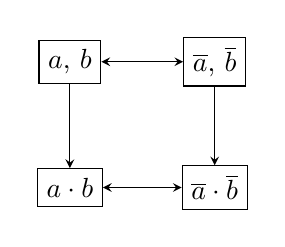
\begin{tikzpicture}[>=stealth]
    \tikzstyle{dom}=[rectangle,draw=black,thin,align=center]

    \node[matrix, column sep=1cm, row sep=1cm](matrix){
      \node[dom](intd){$a$, $b$}; & \node[dom](montd){$\overline{a}$, $\overline{b}$}; \\
      \node[dom](intpro){$a \cdot b$}; &\node[dom](montpro){$\overline{a} \cdot \overline{b}$}; \\
    };

    \draw[<->] (intd) -- (montd);
    \draw[->] (montd) -- (montpro);
    \draw[<->] (montpro) -- (intpro);
    \draw[->] (intd) -- (intpro);
  \end{tikzpicture}
  \caption{Montgomery product flow}
  \label{fig:montpro_flow}
\end{figure}

\filbreak

\section{Turing Machine}

A Turing machine is a mathematical model of computation \cite{Turing}.
Informally, it consists of:
\begin{itemize}
\item A tape divided into cells
\item A head that reads and writes
\item A finite table (action table or transition function)
\item A state
\end{itemize}

\begin{figure}[hbt!]
\centering
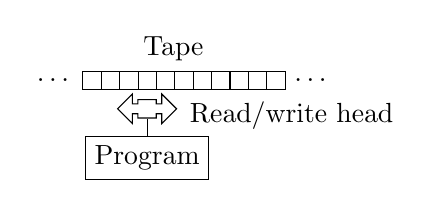
\begin{tikzpicture}[
      start chain=1 going right,start chain=2 going below,node distance=-0.15mm
    ]
    \node [on chain=2] {Tape};
    \node [on chain=1] at (-1.5,-.4) {\ldots};  
    \foreach \x in {1,2,...,11} {
        \x, \node [draw,on chain=1] {};
    } 
    \node [name=r,on chain=1] {\ldots}; 
    \node [name=k, arrow box, draw,on chain=2,
        arrow box arrows={east:.25cm, west:0.25cm}] at (-0.335,-.65) {};    
    \node at (1.5,-.85) {Read/write head};
    \node [on chain=2] {};
    \node [draw,on chain=2] {Program};
    \chainin (k) [join];
\end{tikzpicture}
\caption{Turing machine}
\label{fig:turing}
\end{figure}

A more formal definition comes from Hopcroft \cite{Hopcroft}. A Turing machine
is defined as a 7-tuple $M = \left< Q, \Gamma, b, \Sigma, q_0, F, \delta \right>$
\begin{itemize}
\item $Q$ is a finite, non-empty set of states
\item $\Gamma$ is a finite, non-empty set of the tape alphabet/symbols
\item $b \in \Gamma$ is the blank smybol
\item $\Sigma \subseteq \Gamma \setminus \{ b \}$ the set of input symbols
\item $q_0 \in Q$ is the initial state
\item $F \subseteq Q$ is the set of final or accepting states
\item $\delta : Q \setminus F \times \Gamma \rightarrow Q \times \Gamma \times \{ L,R \}$ is the transition relation
\end{itemize}

\section{Zero Knowledge Proofs of Knowledge}

Sometimes one party wants to prove knowing a secret to the other party
but without actually revealing that secret. Let's take a corporate
espionage example. Suppose that we wish to buy a secret but are not
convinced of the seller's honesty (he may leave us without money and
run away with our secret). We then devise a protocol by which we can
be convinced that the seller knows the secret.

\filbreak

To define a proof a knowledge it is convenient to use a Turing
machine. In this case let's define an interactive Turing machine (ITM)
with 5 tapes:
\begin{itemize}
\item Input tape (read-only)
\item Receiving tape (read-only)
\item Sending tape (write-only)
\item Output tape (write-only)
\item Working tape (read-write)
\end{itemize}

An interactive protocol is an ordered pair of ITMs that share the same
input tape, and have receiving and sending tapes cross-connected
(sending to receiving, receiving to sending).

An interactive proof system can be represented by the following two
properties:
\begin{itemize}
\item Completeness $(x,w) \in \mathcal{R} \Rightarrow P(accept) > \frac{2}{3}$
\item Soundness $(x,w) \notin \mathcal{R} \Rightarrow P(accept) < \frac{1}{3}$
\end{itemize}

Informally, the previous two properties state that
\begin{itemize}
\item if a statement is true, a honest prover will be able to convince the verifier of the validity with a large probability
\item if a statement is false, no dishonest prover will be able to convince the verifier of the validity with a probability larger than the threshold
\end{itemize}

To make it a zero-knowledge an additional property is needed. We can
state that the prover should not release any knowledge on the secret
it possesses. To make it more formal, we state that a third party
should not be able to distinguish between a successful communication
and an unsuccessful one. Depending on how indistinguishable it is, we
can differentiate three cases:
\begin{itemize}
\item perfectly indistinguishable
\item statistically indistinguishable
\item computationally indistinguishable
\end{itemize}

\section{Data Flow Graph and Control Flow Graph}

An algorithm is completely and uniquely defined by its Data Flow Graph (DFG),
whereas the implementation of an algorithm is what gives it its Control Flow
Graph (CFG).

The usual step in converting an algorithm in software to an algorithm
in hardware is to extract the DFG \cite{Schaumont}.

%%% Local Variables: 
%%% TeX-PDF-mode: t
%%% TeX-master: "thesis"
%%% End: 


\section{Tools}
\label{sec:tools}
In this Section we introduce the different tools that conform the core
of our ZKPK framework. These include the LLVM compiler suite and the
GEZEL hardware description language.
%-	ANTLR
%-	LLVM
%-	GEZEL



\subsection{LLVM: A Compiler Framework}
\label{llvm}

LLVM\footnote{http://llvm.org} is a compiler framework designed to
support transparent, life-long program analysis and transformation for
arbitrary programs, by providing high-level information to compiler
transformations at compile-time, link-time, run-time, and in idle time
between runs \cite{LLVM:CGO04}.

Traditional compilers were tailored for only a few languages (with the
exception of GCC). However, all traditional compilers suffer from the
large inter-dependency of the basic blocks (Front-end, Optimizer,
Back-end). LLVM tries to solve this by providing an intermediate form
called the LLVM IR. A typical flow involving the basic blocks is
depicted in Figure \ref{fig:llvm_flow}.

\begin{figure}[hb!]
  \centering
   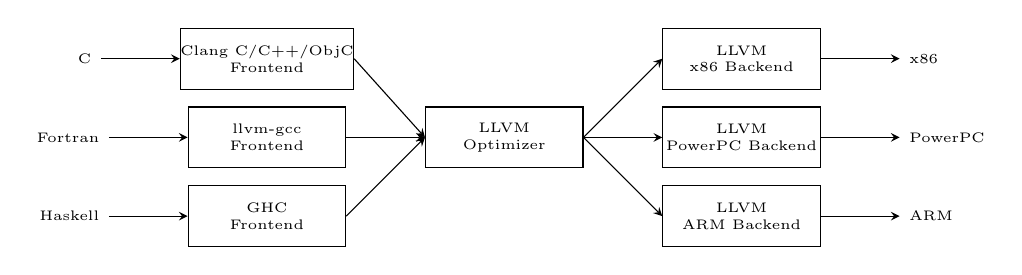
\begin{tikzpicture}[>=stealth]
    \tikzstyle{lang}=[rectangle,draw=black,thin,font=\tiny,inner
    sep=0pt, align=center,minimum width=2cm,minimum height=2.2em]

    \tikzstyle{txt}=[font=\tiny]

    \node[lang](llvm_opt){LLVM \\ Optimizer};
    \node[lang](ppc_back)[right=1 cm of llvm_opt]{LLVM \\ PowerPC Backend};
    \node[txt](ppc)[right=of ppc_back]{PowerPC};
    \node[lang](x86_back)[above of=ppc_back]{LLVM \\ x86 Backend};
    \node[txt](x86)[right=of x86_back]{x86};
    \node[lang](arm_back)[below of=ppc_back]{LLVM \\ ARM Backend};
    \node[txt](arm)[right=of arm_back]{ARM};

    \node[lang](gcc_front)[left=1 cm of llvm_opt]{llvm-gcc \\ Frontend};
    \node[txt](fortran)[left=of gcc_front]{Fortran};
    \node[lang](clang_front)[above of=gcc_front]{Clang C/C++/ObjC \\ Frontend};
    \node[txt](c)[left=of clang_front]{C};
    \node[lang](ghc_front)[below of=gcc_front]{GHC \\ Frontend};
    \node[txt](haskell)[left=of ghc_front]{Haskell};

    \draw[->] (clang_front.east) -- (llvm_opt.west);
    \draw[->] (gcc_front.east) -- (llvm_opt.west);
    \draw[->] (ghc_front.east) -- (llvm_opt.west);

    \draw[->] (llvm_opt.east) -- (x86_back.west);
    \draw[->] (llvm_opt.east) -- (ppc_back.west);
    \draw[->] (llvm_opt.east) -- (arm_back.west);

    \draw[->] (x86_back) -- (x86);
    \draw[->] (ppc_back) -- (ppc);
    \draw[->] (arm_back) -- (arm);

    \draw[->] (c) -- (clang_front);
    \draw[->] (fortran) -- (gcc_front);
    \draw[->] (haskell) -- (ghc_front);
  \end{tikzpicture}
  \caption{LLVM typical workflow \cite{llvm_general}}
  \label{fig:llvm_flow}
\end{figure}

\subsubsection{LLVM IR.}

The LLVM IR is the intermediate representation language of the LLVM
project. On its own it is a first-class language with well defined
semantics \cite{llvm_general,llvmmasterthesis}. Variables are in the SSA (Static Single
Assignment) form meaning that they can only be assigned once and they
keep that value for their entire lifetime. All the values residing in
memory need to be loaded to a variable first and stored back to memory
if they wish to be saved. Instructions operate solely upon
variables. In this respect, the LLVM IR resembles the assembly
language of an infinitely many registers Load-Store based RISC
processor.

The central concept in constructing LLVM IR is the Module. Each module
consists of functions, global variables and symbol table entries.
Modules can be combined using the LLVM linker \cite{llvm_ir}.

\subsection{GEZEL: A Hardware Description Language}
\label{gezel}

GEZEL\footnote{http://rijndael.ece.vt.edu/gezel2/} is a cycle-accurate hardware description language (HDL) using the
Finite-State-Machine + Datapath (FSMD) model. The basic element is a Signal Flow Graph (SFG). It groups operations that
are to be executed concurrently in the same clock cycle. One or more of these SFGs are used to form a datapath, which is the
main building block. A datapath is the smallest GEZEL unit that can stand on
its own and be simulated. Datapaths can be thought of as
\emph{modules} in Verilog or \emph{entities} in VHDL.

Figure \ref{fig:gezel_workflow} shows how the GEZEL language
can be used as an input to the following tools: \emph{fdlvhd}, a generator that can output synthesizeable VHDL or Verilog code; \emph{fdlsim}, a cycle accurate simulator used to verify and validate the design; and \emph{gplatform}, a co-simulation tool used for HW/SW co-design purposes.

\begin{figure}[hb!]
  \centering
  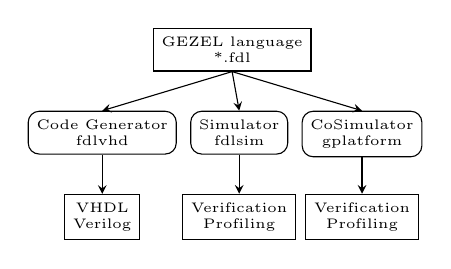
\begin{tikzpicture}[>=stealth, font=\tiny]
    \tikzstyle{edge from parent}=[draw,->]

    \Tree[.\node[language](fdl){GEZEL language \\ *.fdl};
      [.\node[compiler](fdlvhd){Code Generator \\ fdlvhd};
        [.\node[language](vhdl){VHDL \\ Verilog};]
      ]
      [.\node[compiler](fdlsim){Simulator \\ fdlsim};
        [.\node[language](sim){Verification \\ Profiling};]
      ]
      [.\node[compiler](gplatform){CoSimulator \\ gplatform};
        [.\node[language](cosim){Verification \\ Profiling};]
      ]
    ]
  \end{tikzpicture}
  \caption{GEZEL workflow}
  \label{fig:gezel_workflow}
\end{figure}

The co-simulation tool allows to cosimulate GEZEL designs with
instruction-set simulations. Supported processors include
ARM, AVR, 8051, MicroBlaze and PicoBlaze. The cosimulation tool allows
for designing a processor-coprocessor pair for a general purpose
processor and a custom dedicated coprocessor~\cite{Schaumont}.

%%% Local Variables:
%%% TeX-PDF-mode: t
%%% TeX-master: "main"
%%% End:


\section{Custom Framework}
In this section we describe the main functionalities of our
framework. We first give an overview of our proposed solution, and
then we detail the concrete extensions we have performed on the PIL
language. The description of the PIL Front-End and the target
Back-Ends are also covered in this section.
\label{customframework}

\subsection{Framework Overview}
\label{frameworkoverview}
We propose a custom ZPKP compiler framework that takes a protocol
implementation in PIL as generated by the CACE ZKPK compiler and
produces GEZEL or C+GMP code. This allows exploring both ends of the
hardware-software co-design spectrum.
Figure~\ref{fig:custom_framework_workflow} gives an overview of the
custom framework.

\begin{figure}[hb!]
  \centering
  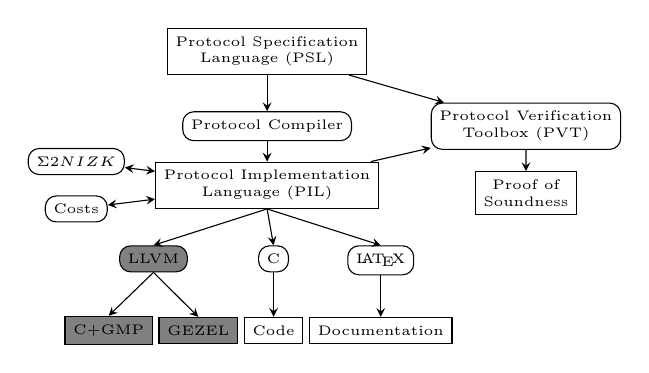
\begin{tikzpicture}[>=stealth,level distance=0.85cm, font=\tiny]
    \tikzstyle{edge from parent}=[draw,->] \tikzset{every leaf
      node/.style={anchor=center}}

    \Tree [.\node[language](psl){Protocol Specification \\ Language (PSL)};
      [.\node[compiler](pc){Protocol Compiler};
        [.\node[language](pil){Protocol Implementation \\ Language (PIL)};
          [.\node[compiler,added](llvm){LLVM};
            \node[language,added](asm){C+GMP};
            \node[language,added](gezel){GEZEL};
          ]
          [.\node[compiler](c){C}; \node[language](code){Code};]
          [.\node[compiler](latex){\LaTeX}; \node[language](doc){Documentation};]
        ]
      ]
    ]

    \node[compiler] (pvt)         [right=of pc,anchor=west]          {Protocol Verification \\ Toolbox (PVT)}
    child {node[language] {Proof of \\ Soundness}};

    \node[compiler] (sigma) [left=of pil.north west,anchor=center] {$\Sigma 2 N I Z K$};
    \node[compiler] (cost) [left=of pil.south west,anchor=center] {Costs};

    \draw[<->] (sigma) -- (pil);
    \draw[<->] (cost) -- (pil);

    \draw[->] (psl) -- (pvt);
    \draw[->] (pil) -- (pvt);
  \end{tikzpicture}
  \caption{Custom framework (extensions to CACE Zero Knowledge
    Compiler highlighted)}
  \label{fig:custom_framework_workflow}
\end{figure}

The generated code from the CACE ZKPK compiler is linked with a
supporting library that is not suitable for small-embedded
devices. The supporting library uses GMP but adds additional
complexity atop. Additionally, our extensions to PIL make it
incompatible with CACE ZKPK compiler.

In order to allow compatibility and improve performance we provide a
software back-end via GMP as well. In our case, there is no added
complexity or semantics. Additionally, we note that these basic GMP
semantics allow us to emulate a target supporting arbitrary-precision
arithmetic.

LLVM was chosen as the compiler framework to transform ZKPK
implementations in PIL into implementations in the desired
languages. The worfklow is depicted in Figure
\ref{fig:custom_llvm_workflow}. The starting point is a ZKPK
implementation in PIL. This implementation is processed by a PIL
Front-end, described in Section~\ref{pilfrontend}, which generates
LLVM IR code. The implementation in LLVM IR can then be used as a
starting point for multiple targets. The LLVM framework provides
back-ends for architectures such as x86, PowerPC and
ARM\footnote{Unfortunately, we cannot use these targets as they do not
  support arbitrary precision arithmetic}. Section~\ref{gezelbackend}
describes the C+GMP and GEZEL back-ends, along with some extensions to GEZEL. Extensions to PIL are 
described in Section~\ref{extensionsPIL}.
\begin{figure}[hb!]
  \centering
  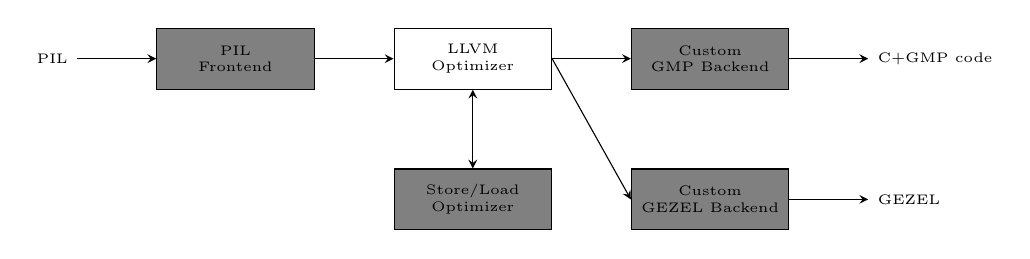
\begin{tikzpicture}[>=stealth]
    \tikzstyle{lang}=[rectangle,draw=black,thin,font=\tiny,inner
    sep=0pt, align=center,minimum width=2cm,minimum height=2.2em]

    \tikzstyle{txt}=[font=\tiny]

    \node[lang](llvm_opt){LLVM \\ Optimizer};

    \node[lang,added](gmp_back)[right=1 cm of llvm_opt]{Custom \\ GMP Backend};
    \node[txt](gmp)[right=of gmp_back]{C+GMP code};

    \node[lang,added](gezel_back)[below=of gmp_back]{Custom \\ GEZEL Backend};
    \node[txt](gezel)[right=of gezel_back]{GEZEL};

    \node[lang,added](llvm_storeloadopt)[below=1 cm of llvm_opt]{Store/Load \\ Optimizer};

    \node[lang,added](pil_front)[left=1 cm of llvm_opt]{PIL \\ Frontend};
    \node[txt](pil)[left=of pil_front]{PIL};

    \draw[->] (pil_front.east) -- (llvm_opt.west);

    \draw[->] (pil) -- (pil_front);

    \draw[->] (llvm_opt.east) -- (gezel_back.west);
    \draw[->] (llvm_opt.east) -- (gmp_back.west);

    \draw[->] (gezel_back) -- (gezel);
    \draw[->] (gmp_back) -- (gmp);

    \draw[<->] (llvm_opt) -- (llvm_storeloadopt);
  \end{tikzpicture}
  \caption{LLVM custom workflow (changes highlighted)}
  \label{fig:custom_llvm_workflow}
\end{figure}


%\subsection{Extensions to CACE Zero-Knowledge Proofs Compiler}
%\label{extensions}

\subsection{Extensions to PIL}
\label{extensionsPIL}

\paragraph{Multiple Blocks.}
PIL specifies Prover and Verifier using respective blocks. A block can
comprise several functions, representing each of the protocol
rounds. The execution order of these rounds should also be
specified. Rounds are executed sequentially.

Besides Prover and Verifier, only an additional Common block, which
contains declarations visible to all the blocks, can be
specified. This makes it impossible to implement a multiparty
protocol, such as the DAA~\cite{DBLP:conf/ccs/BrickellCC04}. We allow
multiple blocks via a simple relaxation of the rules.

\paragraph{Global Variable Access.}
To assure the integrity of the variables in PIL, we have constrained
the language such that global variables can only be modified by the
executing round. This allows the global variable to be backed by a
local variable, which represents the value of the global variable for
the entire duration of the round. Only the last modification gets
written back to the global variable. This has the effect of converting
the CFG to a trivial one with a single node. Previously, the
instructions dominated by the value of the load instruction could not
be executed before the load instruction completed. Without the load
instruction, the ordering can again be arbitrary given the DFG is
satisfied.

The global variables are usually stored in a higher-latency, slower
access storage (register or cache or main memory) so this constraint
will actually improve the performance by accessing the global only
once per read or write.

By introducing this constraint we also protect the implementations
from side-channel attacks. The attacker cannot easily deduce the
location of the storage location of the global variable before the
global variable is actually read. Since the read and write need to
happen only once per round, the time available to launch an attack is
very short.

\paragraph{Compile Time/Constant Expressions.} PIL does not allow
constant expressions as parameters of variables. For example, the following code to declare an integer $f$ of length $l_f + l_{phi} + l_H$ is not allowed.
\begin{lstlisting}[language=PIL]
Common (
  Z l_f = 160;
  Z l_phi = 80;
  Z l_H = 160;
) {}
Smartcard (
  Int(l_f + l_phi + l_H) f
) {}
\end{lstlisting}
Without constant expressions, one would need to recompute the values
manually and re-enter them every time a modification is needed, which is prone to errors. Therefore, we provide PIL with this feature.

\paragraph{Type inference.}
Type inference allows to determine the resulting
type of a certain expression and can also be used to omit
a type declaration. The following example illustrates this:
\begin{lstlisting}[language=PIL]
Zmod*(p) b;
x := Random(Int(80));
a := b^x;
\end{lstlisting}
The type of x can be inferred as Int(80) since
the Random function can only return a random value of the provided
type. As for variable a, since the operation of exponentiation is defined as
applying the multiplication operation many times, the type is Zmod*(p). A similar argument holds when multiplying an element
of the additive modular residue group with an integer. Consequently,
type inference is well defined for any acceptable operation in PIL.

\subsection{PIL Front-end}
\label{pilfrontend}

The purpose of the PIL Front-end is to transform PIL code into LLVM IR code. The PIL Front-end flow is depicted in Figure~\ref{fig:pil_frontend_flow}. First, the protocol implementation in PIL is read by the Lexer, which produces input for the Parser. Next, the Parser reads this input and generates an abstract syntax tree (AST). Finally, the AST is given as input to the Codegen tree-walker, which outputs the protocol implementation in LLVM IR.

\begin{figure}[hb!]
  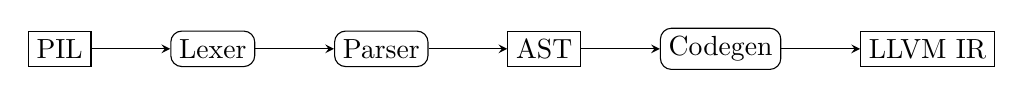
\begin{tikzpicture}[>=stealth]
    \node[language] (pil) {PIL};
    \node[compiler] (lexer) [right=of pil] {Lexer};
    \node[compiler] (parser) [right=of lexer] {Parser};
    \node[language] (ast) [right=of parser] {AST};
    \node[compiler] (codegen) [right=of ast] {Codegen};
    \node[language] (llvm_ir) [right=of codegen] {LLVM IR};

    \draw[->] (pil) -- (lexer);
    \draw[->] (lexer) -- (parser);
    \draw[->] (parser) -- (ast);
    \draw[->] (ast) -- (codegen);
    \draw[->] (codegen) -- (llvm_ir);
  \end{tikzpicture}
  \caption{PIL frontend flow}
  \label{fig:pil_frontend_flow}
\end{figure}

% Both the lexer grammar and the parser grammar are specified in the file pil.g, while the tree-walker and the code generator are
% specified in the file codegen.g. As shown in Figure~\ref{fig:pil_parser_codegen}, ANTLR is used to generate the lexer, the parser and the Codegen tree-walker.
% \begin{figure}[hb!]
%   \centering
%   \subfloat{
%   \begin{tikzpicture}[>=stealth]
%     \tikzstyle{edge from parent}=[draw,->]

%     \Tree[.\node[language](parser_g){pil.g};
%       [.\node[compiler](antlr){ANTLR};
%         [.\node[compiler](lexer){Lexer};]
%         [.\node[compiler](parser){Parser};]
%       ]
%     ]
%   \end{tikzpicture}
%   } \qquad
%   \subfloat{
%   \begin{tikzpicture}[>=stealth]
%     \tikzstyle{edge from parent}=[draw,->]

%     \Tree[.\node[language](tree_g){codegen.g};
%       [.\node[compiler](antlr2){ANTLR};
%         [.\node[compiler](walker){Codegen};]
%       ]
%     ]
%   \end{tikzpicture}
%   }
%   \caption{Lexer, parser and tree walker generation}
%   \label{fig:pil_parser_codegen}
% \end{figure}

The code generation process generates one LLVM module per PIL block.
Every other block except the Common block gets a Common block linked
in. This process is depicted in Figure \ref{fig:linker}.
\begin{figure}[hb!]
  \centering
  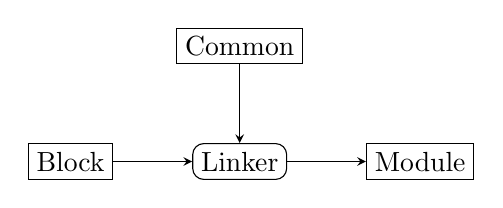
\begin{tikzpicture}[>=stealth]
    \node[language] (block) {Block};
    \node[compiler] (linker) [right=of block] {Linker};
    \node[language] (common) [above=of linker] {Common};
    \node[language] (module) [right=of linker] {Module};

    \draw[->] (block) -- (linker);
    \draw[->] (common) -- (linker);
    \draw[->] (linker) -- (module);
  \end{tikzpicture}
  \caption{Linker}
  \label{fig:linker}
\end{figure}

As result of the transformation, PIL private parameters and global
variables are transformed into LLVM IR global variables, the private
parameters being constant in this case. Each PIL function of a block
is transformed into an LLVM IR function whose input and output
arguments are transformed as such. LLVM's constant folder is used to
evaluate constant time expressions in order to simplify them into a
constant value.

There are two methods to equip LLVM IR with the group types and
arithmetic provided by PIL: either include group types in the core
LLVM files or use the existing IntegerType of LLVM IR and make the
compiler do the extra work. The former allows to preserve the
information about the modular residue groups to the lowest level,
which maintains the security and verifiability of the implementation
to the lowest possible level. However, it requires changes at the core
of the complex LLVM framework, which is error-prone, and it hinders
tracking new LLVM versions if those changes are not integrated into
the main LLVM project.

Therefore, the latter approach was chosen. The group types are backed
by an IntegerType of the appropriate length in the LLVM IR, while type
inference is used to deduce the resulting type of an
operation. Modular operations are transformed into appropriate 3
argument operations with the first 2 arguments being the integer
operands and the third being the modulus.

As result, compatibility with existing LLVM applications is
maintained. The resulting compiler is more complex because it needs to
track types and apply the appropriate operations in the case of group
types. Additionally, if an architecture supports group types (e.g., an
automatic verifier), the workload of its corresponding back-end
increases since now it has to regenerate the lost information
regarding group types.

\subsection{Target Back-ends}
\paragraph{Extensions to GEZEL.}
\label{extensionsGEZEL}

In order to implement modular arithmetic in GEZEL, it is necessary to
follow a two step approach. First, the operation is executed over the
integers, and, second, the modular reduction of the result is
calculated. This approach is valid to implement addition, subtraction
and multiplication, but it cannot be used to support modular
exponentiations.

There are two methods to solve this lack of support: either simulate a
modular exponentiation via implementing it in GEZEL, or extend GEZEL
so that it provides support for modular exponentiation. The latter
approach was taken since it was deemed necessary to enrich the
language with this operation.

\paragraph{GEZEL Back-end.}
\label{gezelbackend}
The GEZEL back-end designs a purely hardware, purely intra-round
combinatorial design. Our PIL semantics allow global variables to be
read at most once and written at most once without any imposed
order. Since there is no enforced order, this allows us to schedule
all the operations in a single clock-cycle.

\paragraph{GMP Back-end.}
\label{gmpbackend}
All of the architectures LLVM supports lack multi-precision arithmetic
support.  This multi-precision support has to come from the software
side via a support library. GMP was chosen as it was deemed the best
option given stability, licensing and performance. The performance
results are due to the efficiency of the GMP library. In this manner,
we take after the CACE ZKPK Compiler.

%%% Local Variables:
%%% TeX-PDF-mode: t
%%% TeX-master: "main"
%%% End:


\section{Discussion}
\label{discussion}

\subsection{Optimizations}

LLVM provides a constant folder which allows constant expressions to
be evaluated at compile time. This eliminates all the redundant calls
that would otherwise be needed at run-time, which can reduce the number
of complex, costly arbitrary-precision operations.

LLVM IR is of the static single assignment form, which allows
aggressive optimizations such as dead-code elimination. Another
advantage of LLVM is the possibility of separating the optimizations
to higher level (common back-end) and lower level (specific back-end).

Since accessing the global variables is slower, writing to the global
variable can be left for the end of the current round or deferred to a
later time, when needed. This allows optimizations in a
hardware-software co-design world where it can be expensive to move
data around.  The optimization is achieved by traversing all the load
instructions that follow a store instruction.  If any of those load
instructions loads from the same location which a store location wrote
to, all the nodes that are dominated by the loaded value are replaced
with the value that was stored. In our model of computation this is
perfectly sane since only the current round can modify a global
variable.

Another optimization example we can think of is exponentiation via
Montgomery multiplications. If we were to translate all the operations
of the algorithm step-by-step, we would have a transfer to the
Montgomery domain, multiplication in the Montgomery domain and return
from the Montgomery domain. The high-level optimizer can eliminate the
unnecessary transfers and returns since they are inverse operations
performed consecutively.

\subsection{Security Analysis}

CACE ZKPK Compiler already offers a formal proof of correctness
covering the transformation from PSL to PIL. We need to analyze the
security of the transformation from PIL to LLVM IR and LLVM IR to the
back-ends whenever possible.

LLVM IR allows us to verify the correctness of the types since LLVM IR
uses code of the static single assignment form, where every variable
is assigned a value exactly once. This allows security assertions to
be taken to a lower level than the one allowed by CACE. 

To assure the correctness of types, first it is necessary to lay out
the DFG of the protocol round. For each node of the DFG preconditions
and postconditions cab be established, such as the ones in Table
\ref{tab:basic_nodes}. Hoare logic~\cite{hoare_logic} can then be
used to prove the correctness of the transformation from PIL to the
LLVM IR.

As for the transformation of LLVM IR into target implementations, it
might not always be possible to prove correctness, especially if the
target implementation is hardware. Since it is impossible to make this
assurance it was deemed unnecessary to go this low and the blocks are
assumed to be correct (if the preconditions are satisfied, the
postconditions will be assured by the block). For the software case,
such properties are assured by the library used.

\begin{table}[h!]
  \centering
  \begin{tabular}{l | c | c}
    Basic block        & Preconditions             & Postconditions \\
    \hline
    Modular adder      & $x \in Z_q^+, y \in Z_q^+$ & $z \in Z_q^+$ \\ 
    Modular multiplier & $x \in Z_p^*, y \in Z_p^*$ & $z \in Z_p^*$ \\
    Zero extender      & $x \in Z_p$               & $z \in Z_p$
  \end{tabular}
  \caption{Basic Nodes}
  \label{tab:basic_nodes}
\end{table}

%%% Local Variables: 
%%% TeX-PDF-mode: t
%%% TeX-master: "main"
%%% End: 


\section{Use Case: Schnorr's Protocol}
\label{schnorr}

The Schnorr's Identification Protocol is a simple
$\Sigma$-protocol. Here we demonstrate how our extensions do not
disrupt the CACE Project ZKC flow but merely complement it. An input
PSL file is given to the CACE Project ZKC and a corresponding PIL file
is received. This PIL file is processed using our framework to
generate both a GEZEL and a GMP target. These are then cross-validated
with the C code that the CACE Project ZKC generates. This was made
possible thanks to the implemented terminal port communication
library.

\subsection{A custom co-processor system}

We took a step further into demonstrating hardware-software co-design
using our framework and have wrote a back-end for an existing
co-processor system. The main processor of this system is an 8051 as
is commonly found on most
smart-cards~\cite{smartcard_crypto_coprocs2}. The 8051 is a very
limited processor and a custom co-processor is needed if cryptography
applications are to be targeted. This leads to a trade-off in terms of
execution time and size as the more operations are implemented in the
co-processor the execution time is lower but the size required is
larger. The project deemed the Montgomery multiplication the most
critical and has implemented it as the only operation on the
co-processor.

The back-end's job was merely to reuse the existing libraries provided
by the co-processor designers but we still believe it was sufficient
to show the feasibility of the approach of this framework. The
execution time was around $2,000,000$ cycles which on a
$\unit[4]{MHz}$ system (common frequency as mentioned in
\cite{smartcard_crypto_coprocs2}) is roughly $\unit[0.5]{s}$.

%%% Local Variables: 
%%% TeX-PDF-mode: t
%%% TeX-master: "paper"
%%% End:


\section{Conclusion and Future Work}
\label{conclusion}
\chapter{Conclusion}

%%% Local Variables: 
%%% TeX-PDF-mode: t
%%% TeX-master: "thesis"
%%% End: 


\bibliographystyle{IEEEtran}
\bibliography{main}

\end{document}

%%% Local Variables: 
%%% TeX-PDF-mode: t
%%% TeX-master: t
%%% End: 
